%&pdflatex
\subsection{Ridimensionare una partizione}
Per ridimensionare una partizione dobbiamo scegliere il partizionamento manuale e, nella schermata successiva, scegliere la partizione da ridimensionare. Nell'esempio, abbiamo selezionato la partizione di Windows 10 (Figura \vref{fig:resize-partition}). Si noti che Windows ha creato 2 partizioni: una da poco più di \texttt{524 MB}, e un'altra da \texttt{53.2 GB} (ovviamente le dimensioni possono essere diverse). La prima partizione (la più piccola) \textbf{non deve essere toccata!}. Se viene modificata, Windows smetterà di funzionare. La seconda partizione (la più grande) è quella che possiamo ridimensionare.

\begin{figure}[ht]
	\centering
	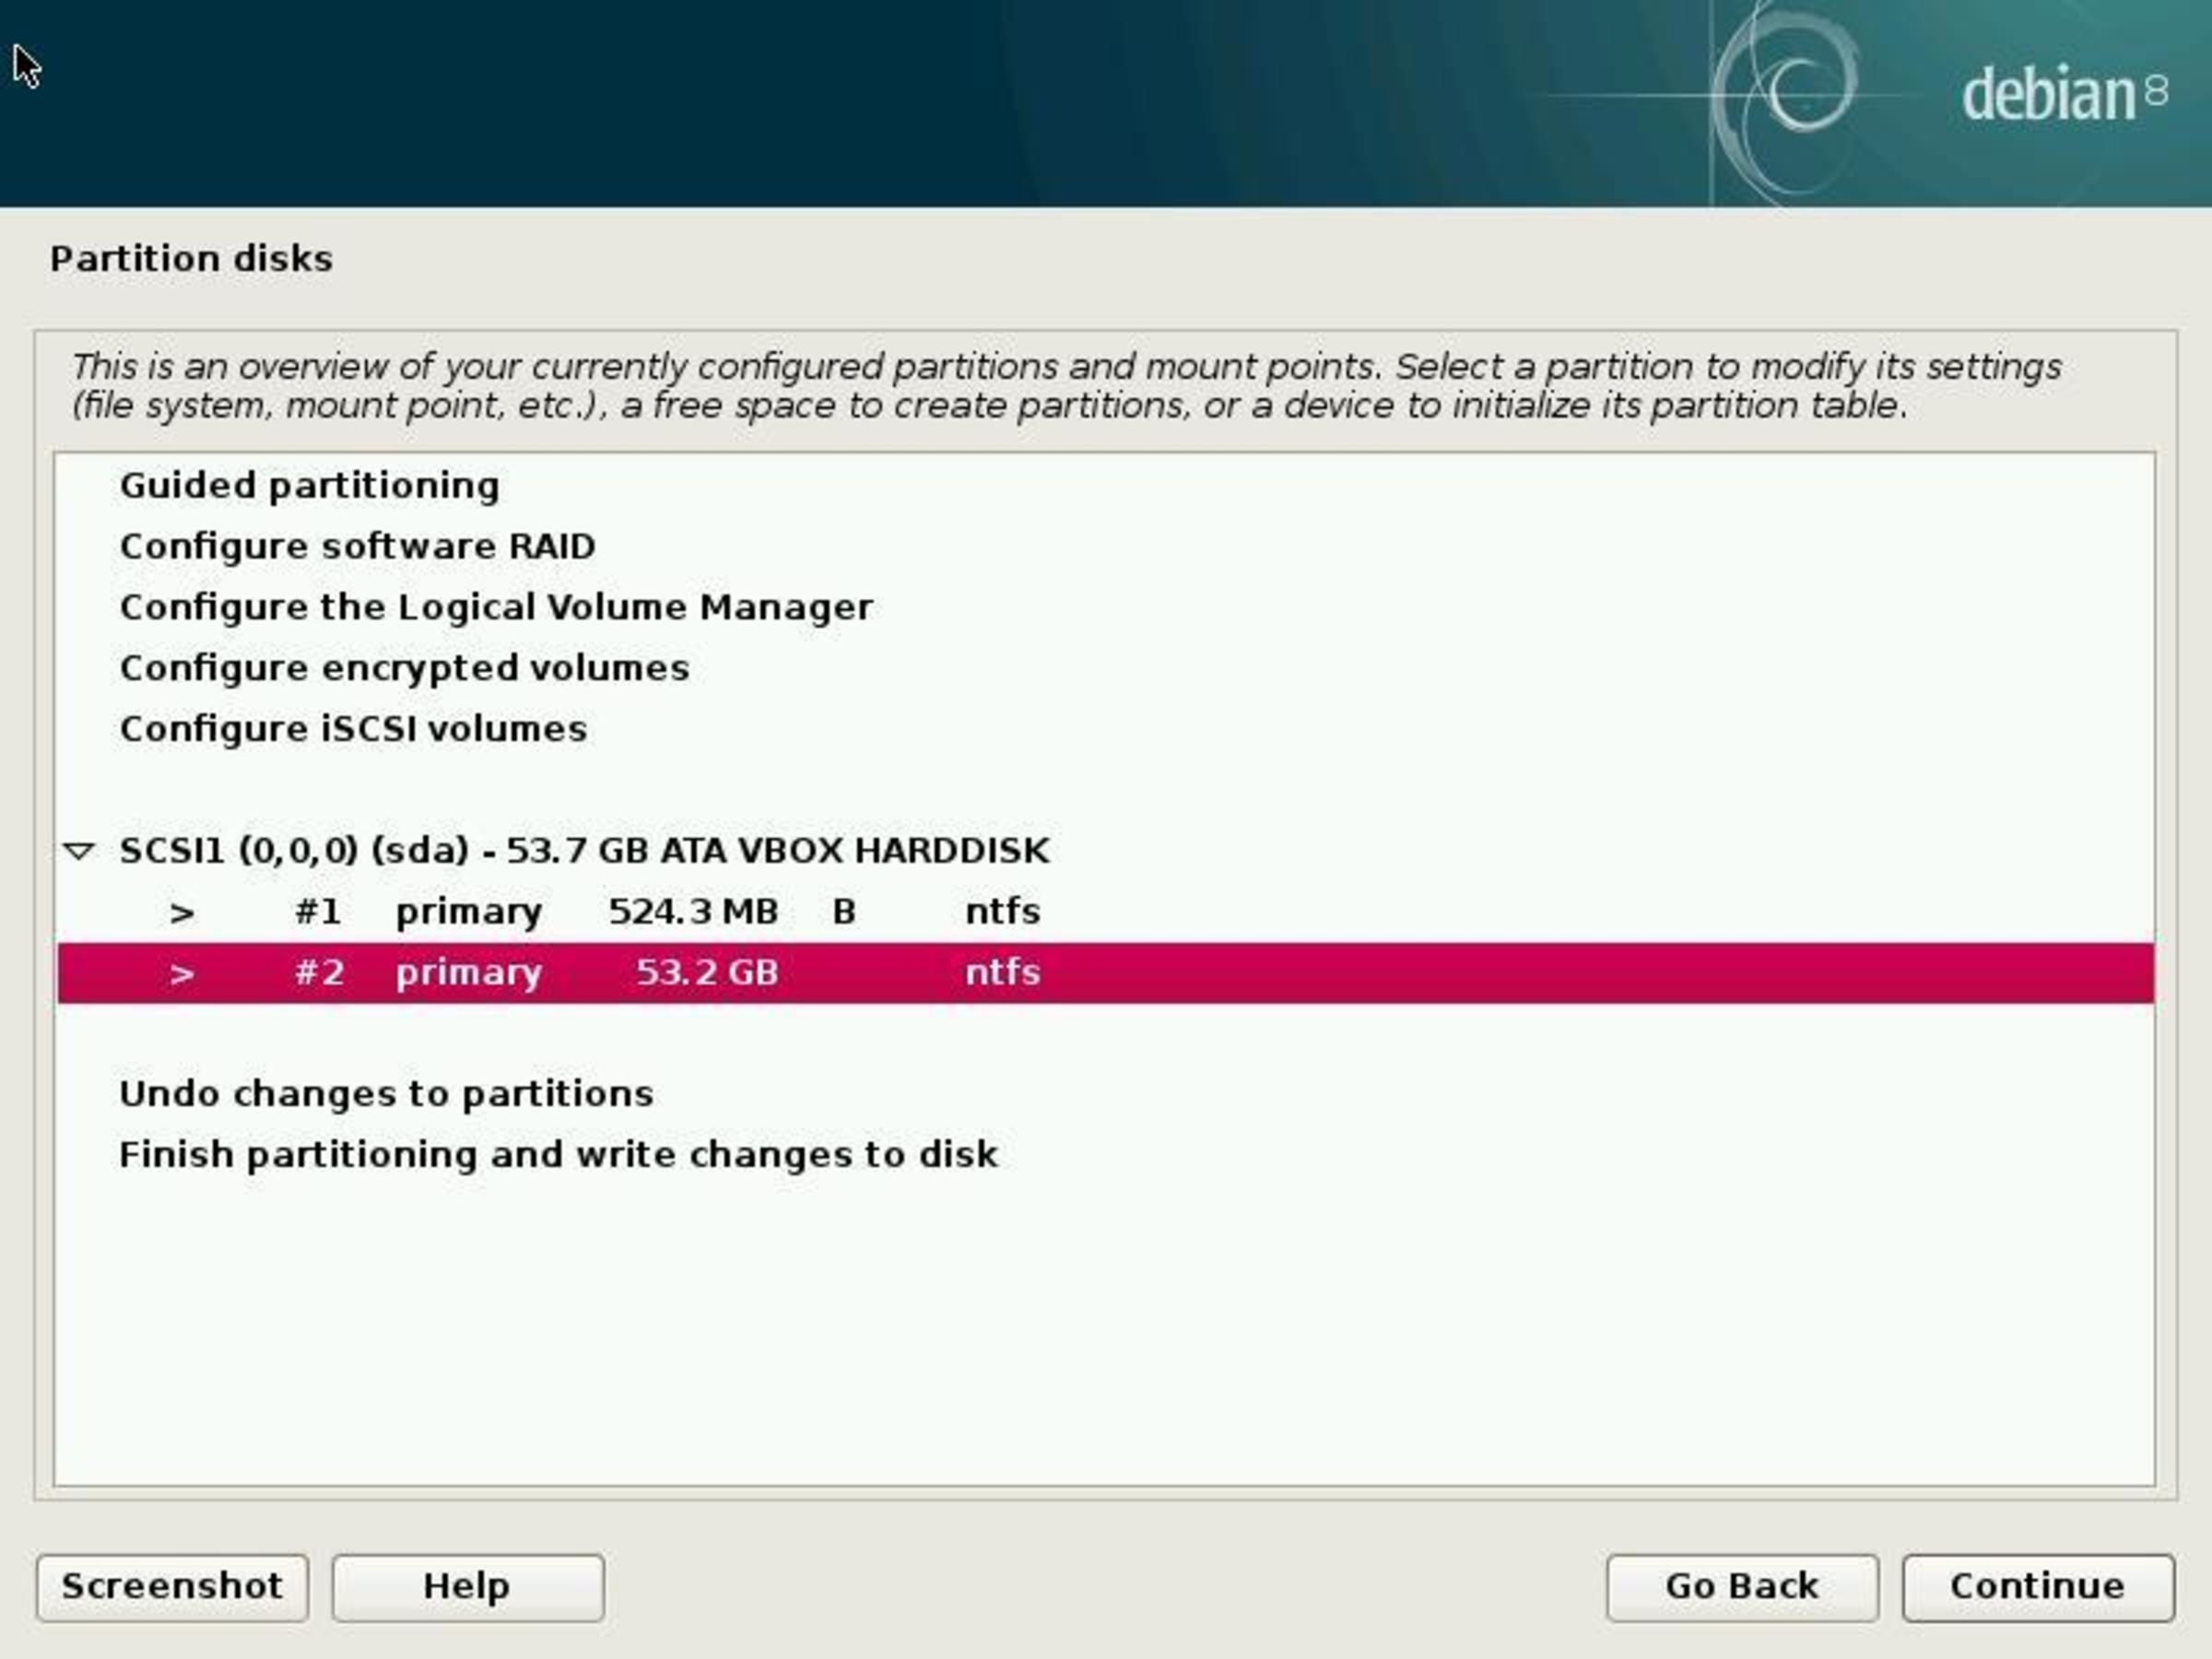
\includegraphics{resize-partition}
	\caption{Selezione della partizione di Windows da ridimensionare}
	\label{fig:resize-partition}
\end{figure}

Dopodiché Debian ci chiederà cosa fare con la partizione selezionata: scegliamo \texttt{Resize the partition} (\texttt{Ridimensionare la partizione}). Quindi ci verrà chiesto di salvare le modifiche fatte finora (anche se non abbiamo ancora fatto nessuna modifica, Debian ce lo chiede comunque): rispondiamo affermativamente con \texttt{Yes} (\texttt{Sì}). Infine, ci verrà chiesta la nuova dimensione per la partizione: consigliamo di riservare almeno \texttt{30 GB} per Debian, e quindi di ridurre la partizione di almeno \texttt{30 GB} rispetto alla dimensione originale.

Al termine ci ritroveremo nella lista delle partizioni: a questo punto dovrebbe essersi generata una quantità di spazio libero sufficiente a contenere Debian (Figura \vref{fig:select-free-space}).
